\hypertarget{metody__sasiedzi_8cpp}{}\section{Dokumentacja pliku metody\+\_\+sasiedzi.\+cpp}
\label{metody__sasiedzi_8cpp}\index{metody\+\_\+sasiedzi.\+cpp@{metody\+\_\+sasiedzi.\+cpp}}
{\ttfamily \#include $<$iostream$>$}\newline
{\ttfamily \#include \char`\"{}klasa\+\_\+element\+\_\+planszy.\+h\char`\"{}}\newline
{\ttfamily \#include \char`\"{}klasa\+\_\+dane\+\_\+planszy.\+h\char`\"{}}\newline
{\ttfamily \#include \char`\"{}klasa\+\_\+plansza.\+h\char`\"{}}\newline
{\ttfamily \#include \char`\"{}klasa\+\_\+sasiedzi.\+h\char`\"{}}\newline
{\ttfamily \#include \char`\"{}klasa\+\_\+element\+\_\+listy\+\_\+sasiadow.\+h\char`\"{}}\newline
{\ttfamily \#include \char`\"{}komunkiaty\+\_\+wyjatki.\+h\char`\"{}}\newline
Wykres zależności załączania dla metody\+\_\+sasiedzi.\+cpp\+:
\nopagebreak
\begin{figure}[H]
\begin{center}
\leavevmode
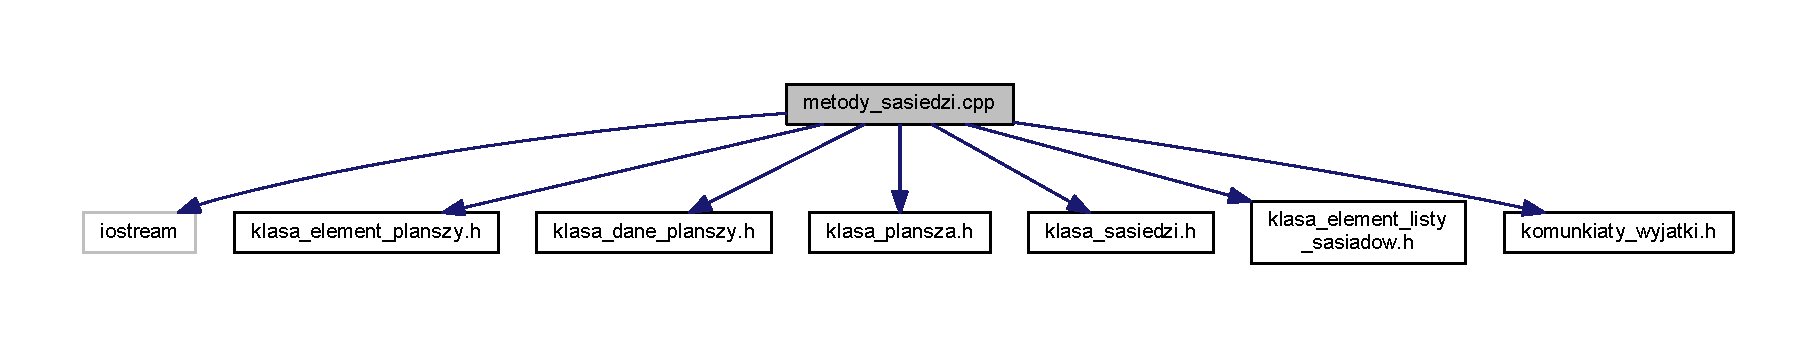
\includegraphics[width=350pt]{metody__sasiedzi_8cpp__incl}
\end{center}
\end{figure}
